El presente capítulo describe el diseño e implementación de la plataforma experimental desarrollada para evaluar el rendimiento y desempeño del aprendizaje de agentes de inteligencia artificial en un entorno de videojuego ejecutado localmente. Se detallan los componentes arquitectónicos, el flujo de comunicación entre módulos, la representación del estado, los mecanismos de registro, el protocolo experimental adoptado y los criterios de viabilidad considerados para evaluar la factibilidad del aprendizaje en distintas condiciones de ejecución.

\section{Arquitectura General del Sistema}

La plataforma se diseñó bajo una arquitectura modular con separación explícita entre el videojuego y los agentes de IA. Esta decisión responde a la necesidad de:

\begin{itemize}
    \item Mantener el juego como fuente única de verdad respecto a reglas.
    \item Permitir el intercambio de agentes sin modificar el motor.
    \item Centralizar la extracción de características.
    \item Garantizar comparabilidad experimental.
\end{itemize}

La arquitectura se compone de tres capas principales:

\begin{enumerate}
    \item \textbf{Videojuego (Unity):} ejecuta las reglas del juego, administra el estado y aplica las acciones.
    \item \textbf{Middleware local:} recibe el estado del juego, procesa la información, enruta la decisión hacia el agente activo y registra métricas.
    \item \textbf{Agentes IA intercambiables:} módulos independientes que implementan una interfaz común de decisión.
\end{enumerate}

Este diseño permite una estructura \textit{plug-and-play}, donde los agentes pueden reemplazarse sin alterar el núcleo del sistema. La Figura~\ref{fig:arquitectura_3capas} presenta la arquitectura general del sistema.

\begin{figure}[H]
\centering
\begin{tikzpicture}[
    block/.style={rectangle, draw, text width=3.8cm, minimum height=2cm, align=center, font=\small},
    arrow/.style={-{Stealth[length=3mm]}, thick},
    label/.style={font=\footnotesize, midway, fill=white, inner sep=1pt}
]
\node[block, fill=blue!15] (unity) {\textbf{Videojuego}\\(Unity / C\#)\\[3pt]Reglas, estado,\\UI, input humano};
\node[block, fill=orange!15, right=2cm of unity] (middleware) {\textbf{Middleware}\\(Python / Flask)\\[3pt]Features, routing,\\logging, métricas};
\node[block, fill=green!15, right=2cm of middleware] (agentes) {\textbf{Agentes IA}\\(Python)\\[3pt]PPO, NEAT, DT,\\KMeans, Heurísticos};

\draw[arrow] (unity.east) -- node[label, above] {estado JSON} (middleware.west);
\draw[arrow] (middleware.west) -- node[label, below] {acción} (unity.east);
\draw[arrow] (middleware.east) -- node[label, above] {obs, legal\_acts} (agentes.west);
\draw[arrow] (agentes.west) -- node[label, below] {PolicyStep} (middleware.east);

\node[below=0.3cm of unity, font=\footnotesize\itshape] {Puerto 8000 (HTTP)};
\node[below=0.3cm of middleware, font=\footnotesize\itshape] {Extracción centralizada};
\node[below=0.3cm of agentes, font=\footnotesize\itshape] {Intercambiables (plug-and-play)};
\end{tikzpicture}
\caption[Arquitectura general del sistema]{Arquitectura general del sistema en tres capas: videojuego, middleware y agentes.}
\label{fig:arquitectura_3capas}
\end{figure}

\section{Formalización Matemática del Entorno}

Con el fin de garantizar reproducibilidad experimental y equivalencia funcional entre el motor de juego y el simulador externo, se define formalmente el entorno de decisión como un sistema determinista basado en función de transición.

\subsection{Definición del Estado}

Sea el estado del entorno:

\[
s = (B_1, B_2, d, t)
\]

donde:

\begin{itemize}
    \item $B_p \in \{0,1,2,3,4,5,6\}^{3 \times 3}$ es el tablero del jugador $p$.
    \item $d \in \{1,\dots,6\}$ es el valor del dado actual.
    \item $t$ es el turno.
\end{itemize}

Cada tablero está compuesto por columnas $C_{p,c}$ con $c \in \{1,2,3\}$.

\subsection{Función de Puntuación}

El puntaje de una columna se calcula sumando, para cada valor único presente en la columna, el producto del valor por el cuadrado de su frecuencia. Sea $U(C_{p,c})$ el conjunto de valores únicos no nulos en la columna $c$ del jugador $p$:

\[
U(C_{p,c}) = \{ v \in \{1,\dots,6\} \mid \exists\, i : B_p[i,c] = v \}
\]

Y sea $f_{p,c}(v)$ la frecuencia del valor $v$ en dicha columna:

\[
f_{p,c}(v) = \left| \{ i \in \{1,2,3\} \mid B_p[i,c] = v \} \right|
\]

Entonces el puntaje de la columna se define como:

\[
Score(C_{p,c}) = \sum_{v \in U(C_{p,c})} v \cdot f_{p,c}(v)^2
\]

Por ejemplo, una columna con valores $[3, 3, 0]$ tiene $U = \{3\}$, $f(3) = 2$, y por tanto $Score = 3 \cdot 2^2 = 12$. Si la columna fuera $[3, 3, 3]$, el puntaje sería $3 \cdot 3^2 = 27$.

El puntaje total del jugador es:

\[
Score(B_p) =
\sum_{c=1}^{3} Score(C_{p,c})
\]

\subsection{Regla de Eliminación}

Al colocar un valor $d$ en la columna $c$ del jugador $p$, se eliminan del tablero rival todas las ocurrencias de $d$ en dicha columna:

\[
B_{\bar{p}}[i,c] =
\begin{cases}
0 & \text{si } B_{\bar{p}}[i,c] = d \\
B_{\bar{p}}[i,c] & \text{en otro caso}
\end{cases}
\]

\subsection{Función de Transición}

Se define la función de transición determinista:

\[
T(s, a) = s'
\]

donde:

\begin{itemize}
    \item $s$ es el estado actual.
    \item $a \in \{0,1,2\}$ es la columna seleccionada.
    \item $s'$ es el estado resultante tras aplicar reglas y actualizar puntuación.
\end{itemize}

Esta formalización permite validar la equivalencia funcional entre el entorno Unity y el simulador Python. La Tabla~\ref{tab:ejemplo_transicion} ilustra un ejemplo concreto de transición.

\begin{table}[H]
\centering
\caption{Ejemplo de transición: el jugador 1 coloca un dado de valor 4 en la columna 1}
\begin{tabular}{lcc}
\hline
\textbf{Elemento} & \textbf{Antes ($s$)} & \textbf{Después ($s'$)} \\
\hline
$B_1$ (tablero propio)   & $\begin{pmatrix} 0 & 3 & 0 \\ 0 & 0 & 5 \\ 0 & 3 & 0 \end{pmatrix}$ & $\begin{pmatrix} 4 & 3 & 0 \\ 0 & 0 & 5 \\ 0 & 3 & 0 \end{pmatrix}$ \\[12pt]
$B_2$ (tablero rival)    & $\begin{pmatrix} 4 & 2 & 0 \\ 0 & 0 & 0 \\ 0 & 6 & 0 \end{pmatrix}$ & $\begin{pmatrix} 0 & 2 & 0 \\ 0 & 0 & 0 \\ 0 & 6 & 0 \end{pmatrix}$ \\[12pt]
Dado $d$ & 4 & --- \\
$Score(B_1)$ & $3 \cdot 2^2 + 5 \cdot 1^2 = 17$ & $17 + 4 = 21$ \\
$Score(B_2)$ & $4 + 2 + 6 = 12$ & $2 + 6 = 8$ \\
\hline
\end{tabular}
\label{tab:ejemplo_transicion}
\end{table}

En este ejemplo, al colocar el dado 4 en la columna 1 del jugador 1, se elimina el valor 4 de la columna 1 del rival (regla de eliminación). El puntaje del rival disminuye de 12 a 8. El puntaje de $B_1$ se calcula como: columna 2 tiene dos 3s ($3 \cdot 2^2 = 12$), columna 3 tiene un 5 ($5 \cdot 1^2 = 5$), total = 17. Después de colocar el 4, se suma $4 \cdot 1^2 = 4$.

\section{Diseño del Entorno de Juego}

Se seleccionó el juego de reglas discretas \textit{Knucklebones}, debido a:

\begin{itemize}
    \item Estado completamente observable.
    \item Número limitado de acciones por turno.
    \item Reglas deterministas y bien definidas.
    \item Facilidad de simulación repetida.
\end{itemize}

Cada turno consiste en:

\begin{itemize}
    \item Recepción de un valor discreto.
    \item Selección de una columna válida.
    \item Aplicación de reglas.
    \item Actualización del puntaje.
\end{itemize}

El entorno garantiza que todos los agentes operen bajo exactamente las mismas condiciones. La Figura~\ref{fig:captura_knucklebones} muestra el prototipo funcional del juego implementado en Unity.

\begin{figure}[H]
\centering
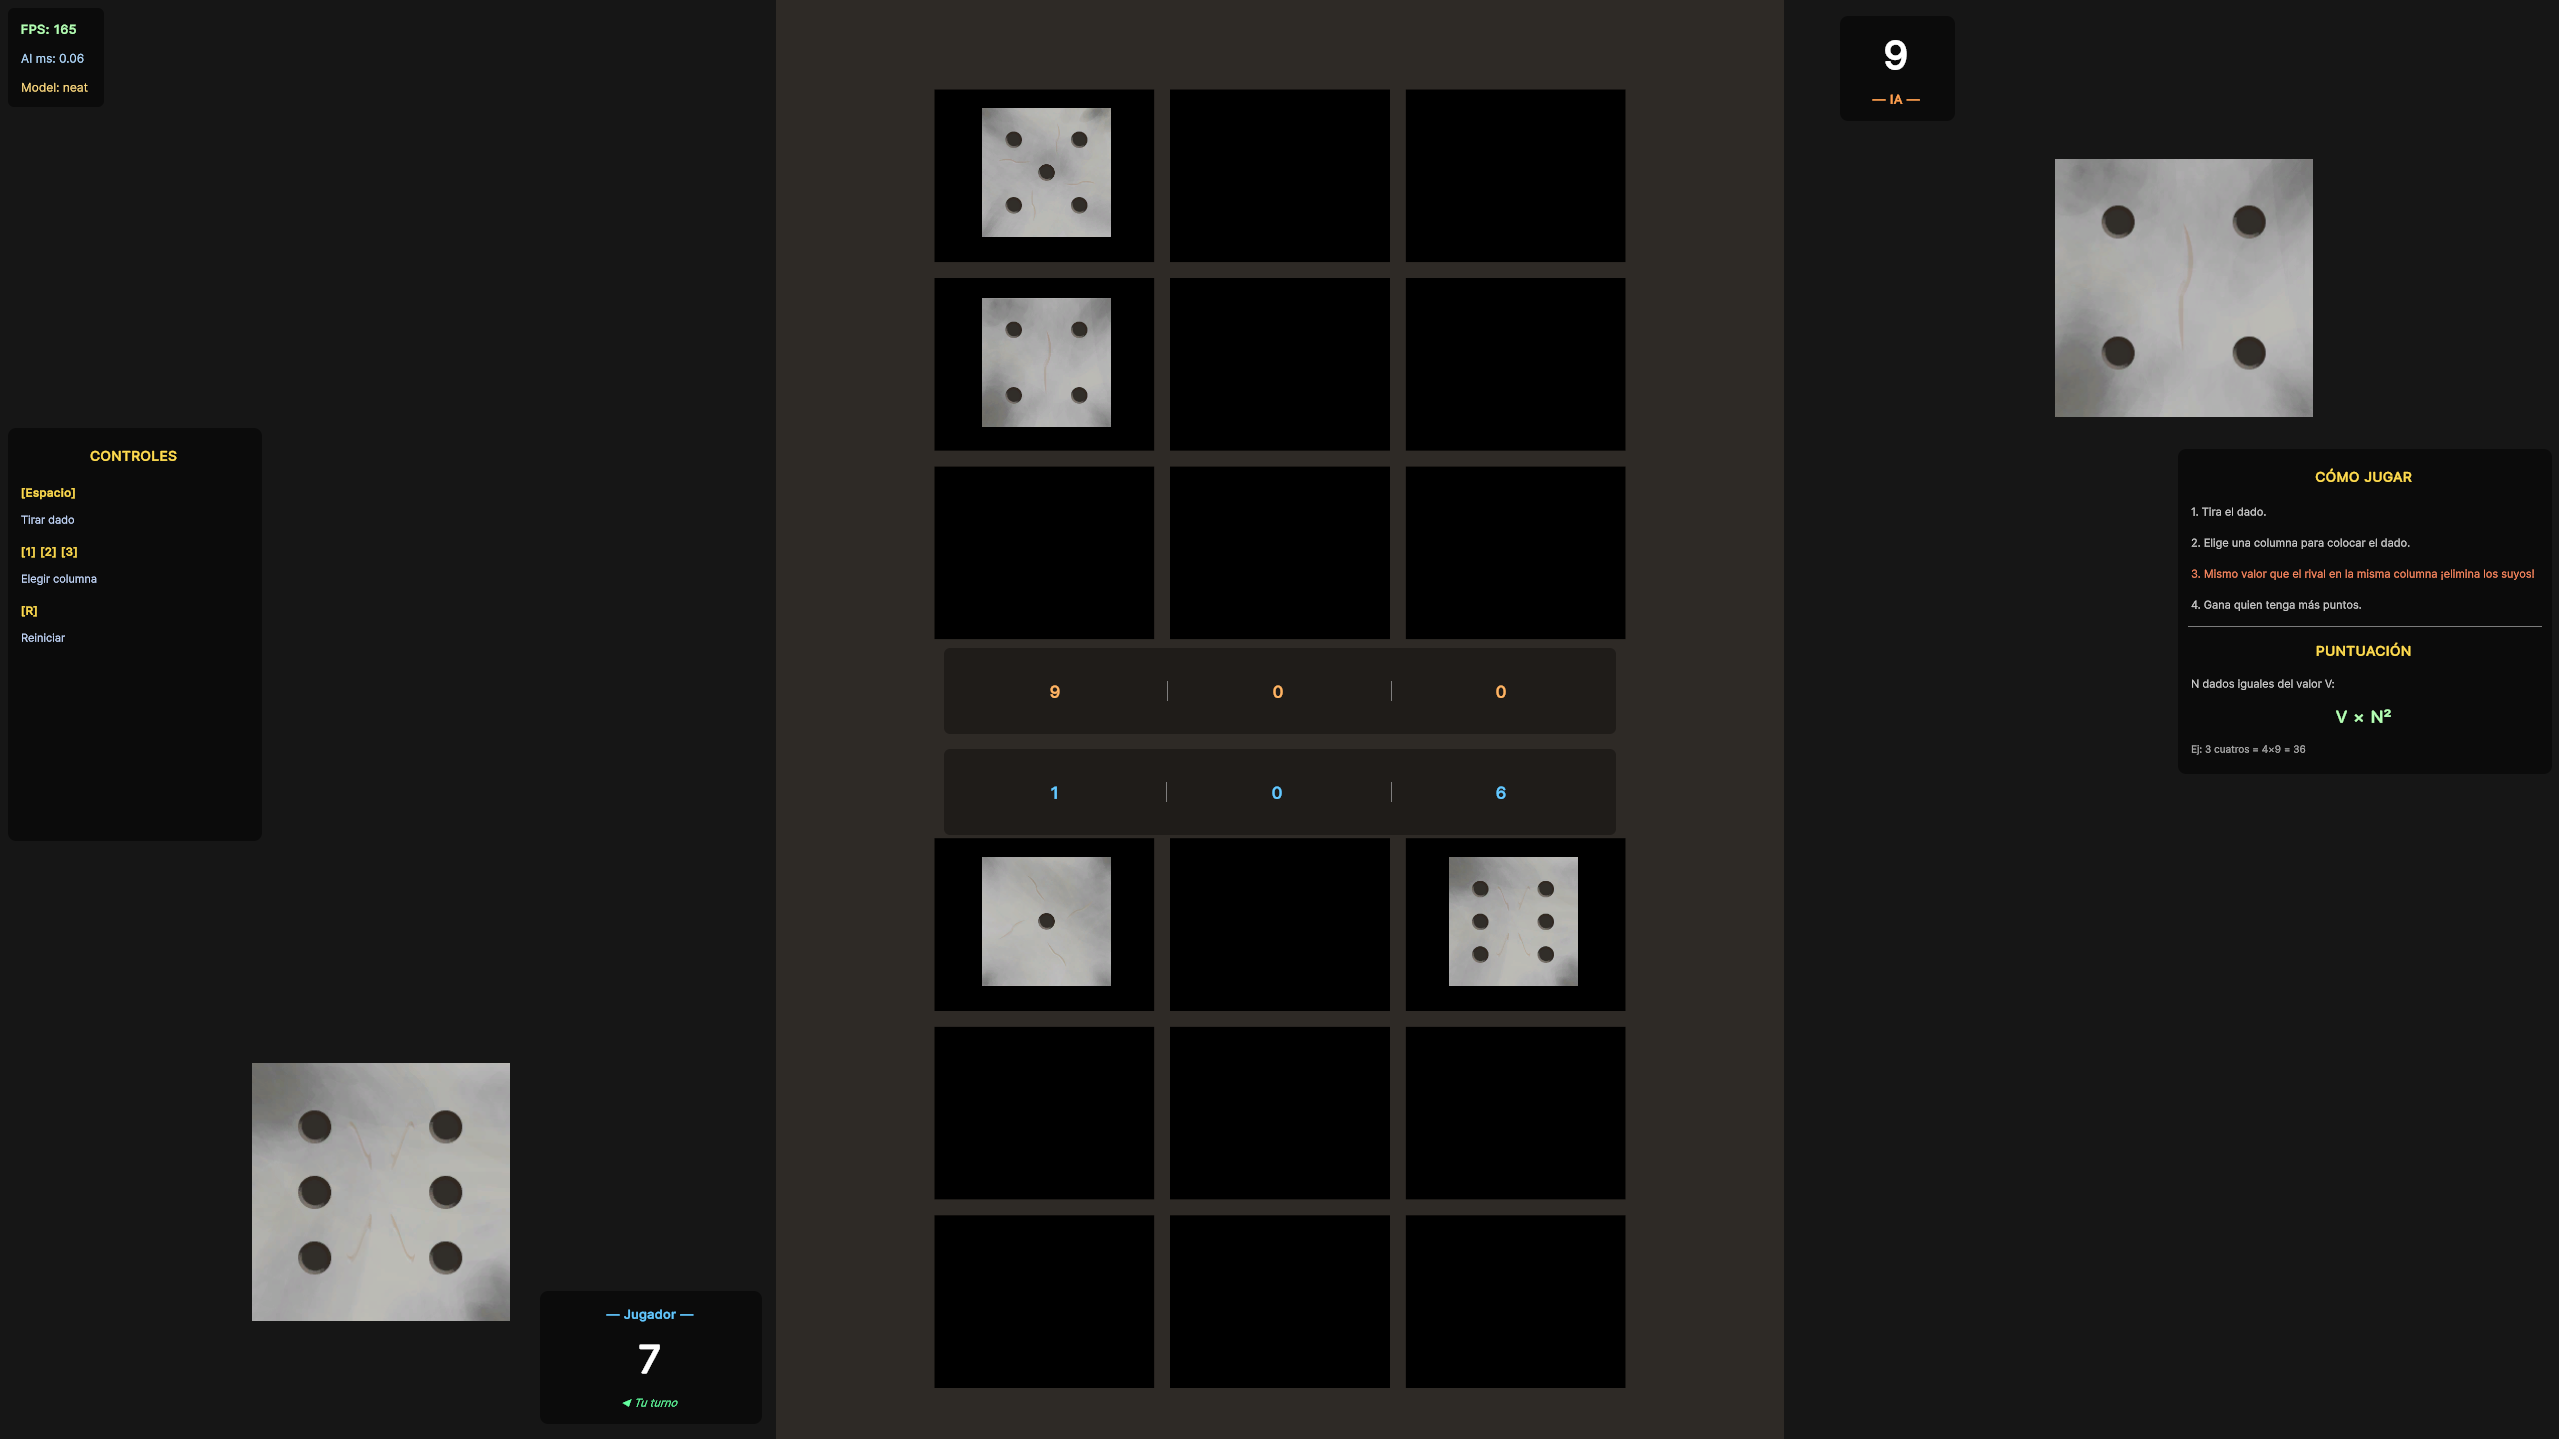
\includegraphics[width=0.85\textwidth]{figures/Knucklebones (3).png}
\caption[Prototipo funcional de Knucklebones en Unity]{Prototipo funcional del juego Knucklebones implementado en Unity con agente de IA externo activo. La interfaz muestra el tablero, el valor del dado actual y las métricas de inferencia utilizadas durante la evaluación del sistema.}
\label{fig:captura_knucklebones}
\end{figure}

\section{Middleware y Comunicación}

La comunicación entre el videojuego y los agentes se realiza mediante un middleware local, utilizando un esquema bloqueante por turno.

El flujo general es:

\begin{enumerate}
    \item El juego emite el estado actual.
    \item El middleware estandariza la representación.
    \item Se extraen características derivadas.
    \item El agente seleccionado retorna una acción.
    \item El middleware registra métricas.
    \item El juego aplica la acción.
\end{enumerate}

Este modelo permite desacoplar completamente la lógica del agente del motor de juego. El flujo de decisión por turno se ilustra en la Figura~\ref{fig:flujo_turno}.

\begin{figure}[H]
\centering
\begin{tikzpicture}[
    flowstep/.style={rectangle, draw, rounded corners, minimum height=0.8cm, minimum width=2.2cm, align=center, font=\footnotesize},
    arrow/.style={-{Stealth[length=2mm]}, thick},
    node distance=0.6cm
]
\node[flowstep, fill=blue!15] (dado) {Tirar dado};
\node[flowstep, fill=blue!15, right=0.5cm of dado] (estado) {Construir\\estado};
\node[flowstep, fill=orange!15, right=0.5cm of estado] (feat) {Extraer\\features (21d)};
\node[flowstep, fill=green!15, right=0.5cm of feat] (agente) {Agente:\\seleccionar\\acción};
\node[flowstep, fill=orange!15, right=0.5cm of agente] (log) {Registrar\\métricas};
\node[flowstep, fill=blue!15, right=0.5cm of log] (aplicar) {Aplicar\\acción};

\draw[arrow] (dado) -- (estado);
\draw[arrow] (estado) -- (feat);
\draw[arrow] (feat) -- (agente);
\draw[arrow] (agente) -- (log);
\draw[arrow] (log) -- (aplicar);

\node[below=0.15cm of dado, font=\tiny\itshape, text=blue!60] {Unity};
\node[below=0.15cm of estado, font=\tiny\itshape, text=blue!60] {Unity};
\node[below=0.15cm of feat, font=\tiny\itshape, text=orange!60] {Middleware};
\node[below=0.15cm of agente, font=\tiny\itshape, text=green!50!black] {Python};
\node[below=0.15cm of log, font=\tiny\itshape, text=orange!60] {Middleware};
\node[below=0.15cm of aplicar, font=\tiny\itshape, text=blue!60] {Unity};
\end{tikzpicture}
\caption[Flujo de decisión por turno]{Flujo de decisión por turno: desde el lanzamiento del dado hasta la aplicación de la acción.}
\label{fig:flujo_turno}
\end{figure}

La Figura~\ref{fig:middleware_real} muestra el middleware en ejecución durante una partida, evidenciando la comunicación activa entre Unity y los agentes Python. Se observa el servidor Flask activo, el sistema cargado y los endpoints expuestos.

\begin{figure}[H]
\centering
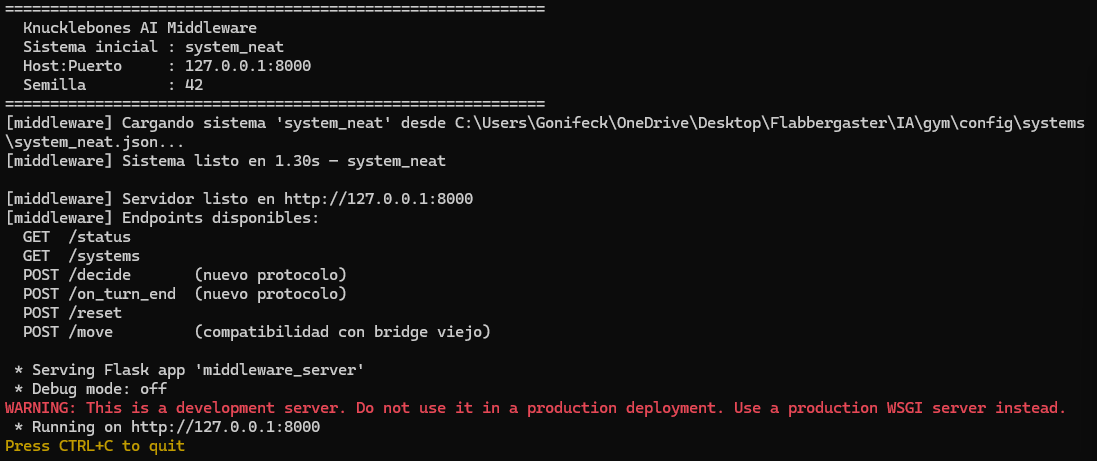
\includegraphics[width=0.75\textwidth]{figures/MiddleWare.png}
\caption[Middleware local en ejecución]{Consola del middleware local en Python. Se observa: (1) el servidor Flask escuchando en el puerto 5000, (2) el sistema adaptativo cargado (system\_neat), y (3) las solicitudes HTTP entrantes desde Unity para los endpoints \texttt{/decide} y \texttt{/status}.}
\label{fig:middleware_real}
\end{figure}

\section{Representación del Estado y Extracción de Características}

Se definió un estado canónico compuesto por:

\begin{itemize}
    \item Tablero propio ($3 \times 3$ valores).
    \item Tablero oponente ($3 \times 3$ valores).
    \item Valor del dado actual.
    \item Puntajes acumulados (propio y rival).
    \item Turno actual.
\end{itemize}

A partir de este estado se calculan 21 características derivadas (features) que alimentan a los agentes de IA. Estas se agrupan en:

\begin{itemize}
    \item \textbf{Características por columna} (3 columnas $\times$ 4 features = 12):
    \begin{itemize}
        \item $ImmediateGain(c)$: incremento de puntaje al colocar el dado en la columna $c$.
        \item $FuturePotential(c)$: potencial de puntuación futura si se completan coincidencias.
        \item $DenialImpact(c)$: reducción del puntaje rival por eliminación de fichas.
        \item $Risk(c)$: exposición a eliminación futura por el rival.
    \end{itemize}
    \item \textbf{Características globales} (9):
    \begin{itemize}
        \item Puntaje propio, puntaje rival, diferencial de puntaje.
        \item Espacios libres por columna (3 valores).
        \item Turno normalizado, ventaja de turno, dado actual normalizado.
    \end{itemize}
\end{itemize}

La centralización del cálculo de características en el middleware evita inconsistencias entre agentes y garantiza que todos operen con la misma representación del estado.

\section{Sistema de Logging e Instrumentación}

Cada turno genera un registro estructurado que incluye:

\begin{itemize}
    \item Estado.
    \item Acción seleccionada.
    \item Agente activo.
    \item Latencia de decisión.
    \item Semilla experimental.
    \item Métricas derivadas.
\end{itemize}

Este registro cumple tres funciones:

\begin{enumerate}
    \item Permitir reconstrucción de partidas.
    \item Construir datasets para entrenamiento supervisado.
    \item Evaluar reproducibilidad experimental.
\end{enumerate}

\section{Control de Aleatoriedad}

Para asegurar comparabilidad entre agentes, se implementó control explícito de semillas (\textit{seed}) para el generador de números aleatorios (RNG).

Esto permite:

\begin{itemize}
    \item Repetir secuencias de juego.
    \item Comparar agentes bajo condiciones idénticas.
    \item Medir estabilidad entre ejecuciones.
\end{itemize}

\section{Entorno de Entrenamiento Equivalente (Gym)}

Debido a restricciones de tiempo y eficiencia de entrenamiento, se desarrolló un entorno equivalente tipo \textit{Gym} que replica las reglas del juego.

Este entorno permite:

\begin{itemize}
    \item Simulación acelerada de partidas.
    \item Generación masiva de datos.
    \item Entrenamiento supervisado o por interacción.
\end{itemize}

El modelo entrenado es posteriormente evaluado bajo el mismo protocolo del entorno principal, garantizando coherencia experimental.

\section{Validación del Simulador Externo}

Dado que el entrenamiento y evaluación de modelos se realiza en un entorno equivalente tipo Gym, fue necesario validar que las reglas implementadas en Python reprodujeran exactamente la lógica del motor Unity.

\subsection{Pruebas de Equivalencia Funcional}

Se generaron trazas de referencia (\textit{golden logs}) desde el entorno Unity, registrando para múltiples turnos:

\begin{itemize}
    \item Estado antes de la acción.
    \item Acción aplicada.
    \item Estado posterior.
    \item Puntajes.
    \item Semilla experimental.
\end{itemize}

Posteriormente, el simulador Python ejecutó la misma secuencia de estados y acciones verificando que:

\[
T_{Unity}(s,a) = T_{Python}(s,a)
\]

para todas las transiciones evaluadas.

La equivalencia exacta de estado posterior garantiza que ambas implementaciones comparten las mismas reglas formales.

\section{Definición Formal de la Política Baseline}

El agente base implementa una política determinista paramétrica basada en combinación ponderada de heurísticas.

Para cada columna disponible $c$ y dado $d$, se calculan:

\begin{itemize}
    \item $ImmediateGain(c,d)$
    \item $FuturePotential(c,d)$
    \item $DenialImpact(c,d)$
    \item $Risk(c,d)$
\end{itemize}

El puntaje compuesto se define como:

\[
ScoreColumn(c,d) =
w_1 ImmediateGain +
w_2 FuturePotential +
w_3 DenialImpact -
w_4 Risk
\]

La acción seleccionada es:

\[
a = \arg\max_c ScoreColumn(c,d)
\]

\subsection{Aleatoriedad Acotada}

Para evitar determinismo absoluto, se introduce un margen relativo $\epsilon$:

\[
\frac{|ScoreColumn(c_i) - ScoreColumn(c_{best})|}{ScoreColumn(c_{best})} < \epsilon
\]

Si múltiples columnas cumplen la condición, se selecciona una aleatoriamente dentro de ese subconjunto.

Esta política constituye el \textit{baseline} contra el cual se comparan los modelos aprendidos.

\subsection{Control de Aleatoriedad}

Para evitar discrepancias en generación de dados, el valor $d$ fue inyectado explícitamente en el simulador durante la validación, eliminando dependencia de generadores RNG internos.

\section{Protocolo Experimental}

Para la evaluación comparativa se definieron:

\subsection{Métricas de desempeño}

\begin{itemize}
    \item Tasa de victoria.
    \item Diferencial de puntaje.
    \item Estabilidad estadística.
\end{itemize}

\subsection{Métricas computacionales}

\begin{itemize}
    \item Latencia promedio de decisión.
    \item Uso de CPU y memoria.
    \item Tiempo de entrenamiento (cuando aplica).
\end{itemize}

Los experimentos se ejecutan con semillas controladas y número fijo de partidas por configuración, permitiendo análisis comparativo reproducible.

\section{Criterios de Viabilidad para Entrenamiento en Tiempo Real}

Un aspecto central de esta investigación es determinar si los paradigmas de aprendizaje evaluados podrían, en principio, ejecutar su proceso de entrenamiento durante una sesión de juego contra un jugador humano, es decir, en tiempo real y en hardware local. Para ello se definen los siguientes criterios de viabilidad, derivados de las condiciones observables en una sesión real de juego.

\subsection{Disponibilidad de datos en una sesión real}

Una partida típica de Knucklebones tiene aproximadamente 18 turnos y dura entre 1 y 3 minutos. Un jugador humano razonablemente comprometido podría jugar entre 10 y 100 partidas antes de perder interés, lo que produce entre 180 y 1,800 muestras de decisión (pares estado-acción). Este volumen se contrasta con los requisitos de entrenamiento de cada paradigma para evaluar la brecha de datos.

\subsection{Requisitos de entrenamiento por paradigma}

\begin{itemize}
    \item \textbf{PPO (Aprendizaje por Refuerzo):} los experimentos utilizaron 400,000 timesteps distribuidos en miles de episodios. Este volumen es varios órdenes de magnitud superior al disponible en una sesión humana.
    \item \textbf{NEAT (Neuroevolución):} el proceso evolutivo requiere evaluar poblaciones completas de genomas durante cientos de generaciones. En la configuración utilizada, cada genoma fue evaluado contra 102 episodios (34 por cada una de 3 semillas), y se mantuvieron poblaciones de 150 genomas durante 300 generaciones, resultando en millones de episodios evaluados en total.
    \item \textbf{DT (Árboles de Decisión destilados):} el entrenamiento supervisado es casi instantáneo ($<$3 segundos), pero depende de un dataset generado por un teacher PPO previamente entrenado. Sin un teacher, no dispone de datos etiquetados.
\end{itemize}

\subsection{Criterio de brecha}

Se define la \textit{brecha de datos} como la relación entre el volumen de datos requerido para obtener un agente funcional y el volumen disponible en una sesión real:

\[
\text{Brecha de datos} = \frac{\text{Datos requeridos para entrenamiento}}{\text{Datos disponibles en sesión real}}
\]

Un valor cercano a 1 indicaría viabilidad; valores de varios órdenes de magnitud indican inviabilidad práctica. Este criterio se evalúa cuantitativamente en el Capítulo~\ref{cap:aplicacion}.

\subsection{Criterio de estabilidad}

Adicionalmente, un modelo que se entrena con datos extremadamente limitados presenta riesgo de:

\begin{itemize}
    \item \textbf{Sobreajuste:} memorizar las pocas partidas observadas en lugar de generalizar.
    \item \textbf{Inestabilidad:} convergencia errática o políticas que varían drásticamente entre ejecuciones.
    \item \textbf{Rendimiento aleatorio:} como se observó en los experimentos con NEAT entrenado con seed fija y pocas generaciones, donde el agente no convergió (WR $\approx$ 0.50, equivalente a aleatorio).
\end{itemize}

Estos criterios permiten evaluar no solo si es posible ejecutar el entrenamiento, sino si el resultado del entrenamiento sería útil bajo las restricciones de una sesión real.

